% ============================================================
%  AWARE Project — Beamer Presentation
%  From Concern to Action: Polarization Interventions in Brazil
% ============================================================
\documentclass[aspectratio=169]{beamer}

\usetheme{Madrid}

% ── IJL brand colour ────────────────────────────────────────
\definecolor{IJLblue}{RGB}{0, 0, 205}
\definecolor{IJLred}{RGB}{180, 30, 30}
\definecolor{macroC}{RGB}{0, 100, 180}
\definecolor{microC}{RGB}{180, 60, 0}

\setbeamercolor{palette primary}   {bg=IJLblue,  fg=white}
\setbeamercolor{palette secondary} {bg=IJLblue!85!black, fg=white}
\setbeamercolor{palette tertiary}  {bg=IJLblue!70!black, fg=white}
\setbeamercolor{palette quaternary}{bg=IJLblue!55!black, fg=white}
\setbeamercolor{structure}         {fg=IJLblue}
\setbeamercolor{frametitle}        {bg=IJLblue, fg=white}
\setbeamercolor{title}             {fg=white}
\setbeamercolor{author in head/foot}{bg=IJLblue!80!black, fg=white}
\setbeamercolor{title in head/foot} {bg=IJLblue!60!black, fg=white}
\setbeamercolor{date in head/foot}  {bg=IJLblue!40!black, fg=white}

% ── Packages ────────────────────────────────────────────────
\usepackage[T1]{fontenc}
\usepackage[utf8]{inputenc}
\usepackage{graphicx}
\usepackage{eso-pic}
\usepackage{booktabs}
\usepackage{multirow}
\usepackage{tikz}
\usetikzlibrary{arrows.meta, positioning, shapes.geometric, fit, backgrounds}
\usepackage{colortbl}
\usepackage{xcolor}
\usepackage{array}
\usepackage{pifont}

% ── Footer ──────────────────────────────────────────────────
\setbeamertemplate{footline}{%
  \leavevmode%
  \hbox{%
    \begin{beamercolorbox}[wd=.08\paperwidth,ht=2.5ex,dp=1.125ex,
        leftskip=.2cm,rightskip=.1cm]{author in head/foot}%
      \raisebox{-0.25ex}{
\includegraphics[height=2.2ex]{IJL-largo-ingles.jpg}}%
    \end{beamercolorbox}%
    \begin{beamercolorbox}[wd=.27\paperwidth,ht=2.5ex,dp=1.125ex,
        leftskip=.1cm,rightskip=.3cm plus1fil]{author in head/foot}%
      \usebeamerfont{author in head/foot}\insertshortauthor
    \end{beamercolorbox}%
    \begin{beamercolorbox}[wd=.50\paperwidth,ht=2.5ex,dp=1.125ex,
        leftskip=.3cm,rightskip=.3cm plus1fil]{title in head/foot}%
      \usebeamerfont{title in head/foot}\insertshorttitle
    \end{beamercolorbox}%
    \begin{beamercolorbox}[wd=.15\paperwidth,ht=2.5ex,dp=1.125ex,
        leftskip=.3cm,rightskip=.3cm]{date in head/foot}%
      \usebeamerfont{date in head/foot}%
      \hfill\insertframenumber{}/\inserttotalframenumber\hspace{0.4em}%
    \end{beamercolorbox}%
  }%
  \vskip0pt%
}
\setbeamertemplate{navigation symbols}{}

% ── Logo overlay: bottom-left, small ────────────────────────
\newcommand{\IJLlogoOverlay}{%
  \AddToShipoutPictureFG{%
    \AtPageLowerLeft{%
      \hspace{0.22cm}%
      \raisebox{0.5cm}{%
        
\includegraphics[height=0.52cm]{IJL-largo-ingles.jpg}%
      }%
    }%
  }%
}

% ── Animated bar chart: biggest problem ─────────────────────
% Bars appear one by one; on overlay 5, all faded except Polarization
% Scale: 0.20 cm/%, bars start at x=4.3cm
% Bar heights 0.42cm, spacing 0.72cm
\newcommand{\problembarchart}{%
  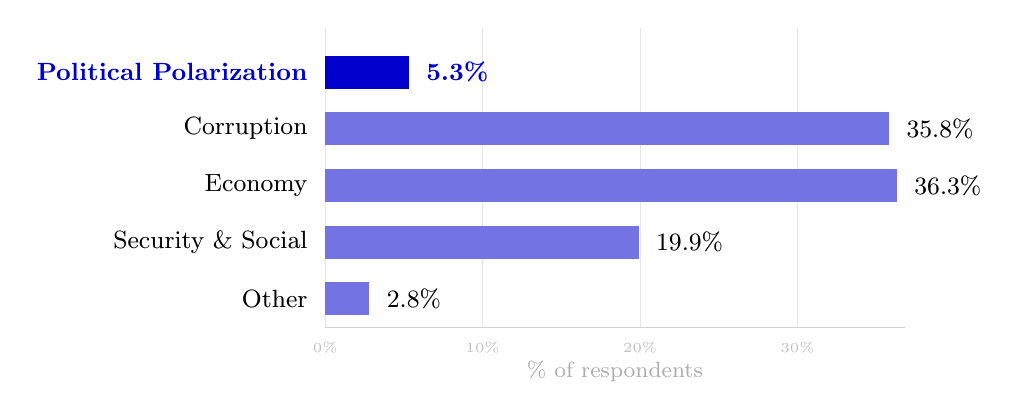
\begin{tikzpicture}
    % Grid lines
    \foreach \xpct/\gx in {0/4.3, 10/6.3, 20/8.3, 30/10.3}{%
      \draw[gray!20, very thin] (\gx,-0.15) -- (\gx,3.65);
      \node[gray!50, font=\tiny, below] at (\gx,-0.22) {\xpct\%};
    }
    \draw[gray!35, thin] (4.3,-0.15) -- (11.66,-0.15);
    % Bar 1: Other 2.8%  — x: 4.3→4.86,  y: 0.00→0.42
    \onslide<1->{%
      \alt<5>{%
        \fill[gray!25] (4.3,0.00) rectangle (4.86,0.42);
        \node[gray!55,font=\small,left]  at (4.2,0.21) {Other};
        \node[gray!55,font=\small,right] at (4.96,0.21) {2.8\%};
      }{%
        \fill[IJLblue!55] (4.3,0.00) rectangle (4.86,0.42);
        \node[font=\small,left]  at (4.2,0.21) {Other};
        \node[font=\small,right] at (4.96,0.21) {2.8\%};
      }%
    }
    % Bar 2: Security & Social 19.9%  — x: 4.3→8.28,  y: 0.72→1.14
    \onslide<2->{%
      \alt<5>{%
        \fill[gray!25] (4.3,0.72) rectangle (8.28,1.14);
        \node[gray!55,font=\small,left]  at (4.2,0.93) {Security \& Social};
        \node[gray!55,font=\small,right] at (8.38,0.93) {19.9\%};
      }{%
        \fill[IJLblue!55] (4.3,0.72) rectangle (8.28,1.14);
        \node[font=\small,left]  at (4.2,0.93) {Security \& Social};
        \node[font=\small,right] at (8.38,0.93) {19.9\%};
      }%
    }
    % Bar 3: Economy 36.3%  — x: 4.3→11.56,  y: 1.44→1.86
    \onslide<3->{%
      \alt<5>{%
        \fill[gray!25] (4.3,1.44) rectangle (11.56,1.86);
        \node[gray!55,font=\small,left]  at (4.2,1.65) {Economy};
        \node[gray!55,font=\small,right] at (11.66,1.65) {36.3\%};
      }{%
        \fill[IJLblue!55] (4.3,1.44) rectangle (11.56,1.86);
        \node[font=\small,left]  at (4.2,1.65) {Economy};
        \node[font=\small,right] at (11.66,1.65) {36.3\%};
      }%
    }
    % Bar 4: Corruption 35.8%  — x: 4.3→11.46,  y: 2.16→2.58
    \onslide<4->{%
      \alt<5>{%
        \fill[gray!25] (4.3,2.16) rectangle (11.46,2.58);
        \node[gray!55,font=\small,left]  at (4.2,2.37) {Corruption};
        \node[gray!55,font=\small,right] at (11.56,2.37) {35.8\%};
      }{%
        \fill[IJLblue!55] (4.3,2.16) rectangle (11.46,2.58);
        \node[font=\small,left]  at (4.2,2.37) {Corruption};
        \node[font=\small,right] at (11.56,2.37) {35.8\%};
      }%
    }
    % Bar 5: Political Polarization 5.3%  — x: 4.3→5.36,  y: 2.88→3.30  (always IJL blue)
    \onslide<5->{%
      \fill[IJLblue] (4.3,2.88) rectangle (5.36,3.30);
      \node[IJLblue,font=\small\bfseries,left]  at (4.2,3.09) {Political Polarization};
      \node[IJLblue,font=\small\bfseries,right] at (5.46,3.09) {5.3\%};
    }
    \node[font=\footnotesize,gray!65,below] at (7.98,-0.45) {\% of respondents};
  \end{tikzpicture}%
}

% ── Metadata ────────────────────────────────────────────────
\title[AWARE: Polarization \& Behavior]{From Concern to Action}
\subtitle{Can Highlighting the Dangers of Polarization Increase Citizens' Willingness to Intervene?\\
\small Evidence from Combined Experiments in Brazil}
\author[Mello, Chauchard, Jurado]{%
  Fernando B.\ Mello\inst{1} \and
  Simon Chauchard\inst{1} \and
  Ignácio Jurado\inst{2}}
\institute[IJL/CSIC]{%
  \inst{1}Universidad Carlos III de Madrid \& Instituto Juan Linz \and
  \inst{2}CSIC
}
\date[2026]{2026}

% ============================================================
\begin{document}

% ── Title slide ─────────────────────────────────────────────
\begin{frame}
  \titlepage
\end{frame}

% ── Table of contents ───────────────────────────────────────
\begin{frame}{Outline}
  \tableofcontents
\end{frame}

% ============================================================
\section{Motivation}
% ============================================================

\begin{frame}{The Problem: Polarization in Contemporary Democracies}
  \begin{columns}[T]
    \column{0.55\textwidth}
      \begin{itemize}
        \item<1-> Affective polarization has risen sharply across democracies — citizens increasingly \textbf{dislike} and \textbf{distrust} the other side
        \item<2-> Polarization \textbf{threatens institutions}: erodes electoral trust, weakens democratic norms, enables democratic backsliding
        \item<3-> Polarization \textbf{damages everyday life}: hostile interactions, family conflict, online aggression
        \item<4-> Brazil is a key case — one of the world's most polarized electorates after 2018
      \end{itemize}
    \column{0.42\textwidth}
      \begin{block}{The Puzzle}
        \smallskip
        People are aware of polarization's costs — yet \textbf{behavioral change remains elusive}.\\[6pt]
        Can \emph{framing} those costs trigger action?
      \end{block}
      \vspace{0.5em}
      \begin{alertblock}{Our Approach}
        \smallskip
        Two parallel experiments targeting \textbf{both} the supply (elites) and demand (citizens) sides simultaneously.
      \end{alertblock}
  \end{columns}
\end{frame}

\begin{frame}{Theoretical Framework}
  \begin{center}
  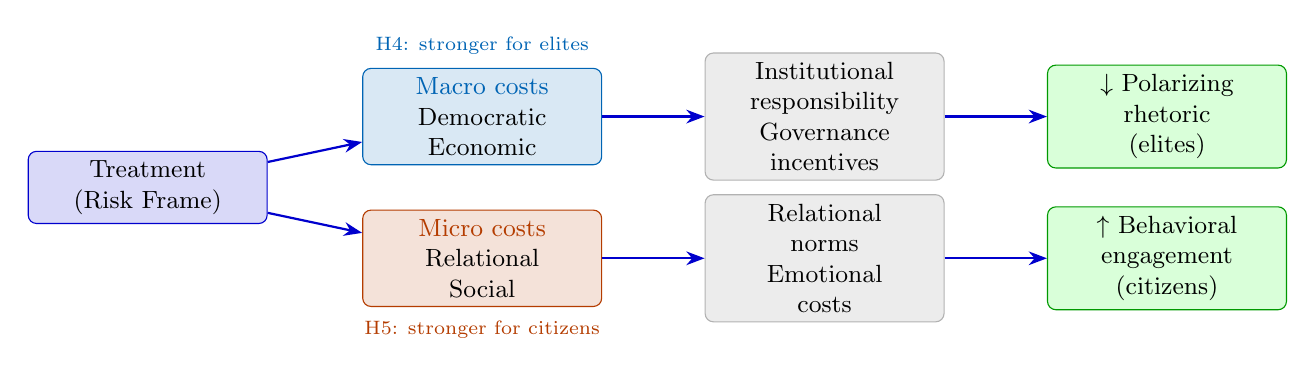
\begin{tikzpicture}[
    node distance=0.6cm and 1.2cm,
    box/.style={rectangle, rounded corners=3pt, draw, minimum height=0.8cm,
                text width=2.8cm, align=center, font=\small},
    arrow/.style={-Stealth, thick, IJLblue},
    every node/.style={font=\small}
  ]
    % Treatment
    \node[box, fill=IJLblue!15, draw=IJLblue] (treat) {Treatment\\(Risk Frame)};

    % Perceived costs
    \node[box, fill=macroC!15, draw=macroC, right=of treat, yshift=0.9cm] (macro)
      {\textcolor{macroC}{Macro costs}\\Democratic\\Economic};
    \node[box, fill=microC!15, draw=microC, right=of treat, yshift=-0.9cm] (micro)
      {\textcolor{microC}{Micro costs}\\Relational\\Social};

    % Mechanisms
    \node[box, fill=gray!15, draw=gray!60, right=1.3cm of macro] (mech1)
      {Institutional\\responsibility\\Governance\\incentives};
    \node[box, fill=gray!15, draw=gray!60, right=1.3cm of micro] (mech2)
      {Relational\\norms\\Emotional\\costs};

    % Outcomes
    \node[box, fill=green!15, draw=green!60!black, right=1.3cm of mech1] (elite)
      {$\downarrow$ Polarizing\\rhetoric\\(elites)};
    \node[box, fill=green!15, draw=green!60!black, right=1.3cm of mech2] (citizen)
      {$\uparrow$ Behavioral\\engagement\\(citizens)};

    % Arrows
    \draw[arrow] (treat) -- (macro);
    \draw[arrow] (treat) -- (micro);
    \draw[arrow] (macro) -- (mech1);
    \draw[arrow] (micro) -- (mech2);
    \draw[arrow] (mech1) -- (elite);
    \draw[arrow] (mech2) -- (citizen);

    % Labels
    \node[above=0.05cm of macro, font=\scriptsize, text=macroC] {H4: stronger for elites};
    \node[below=0.05cm of micro, font=\scriptsize, text=microC] {H5: stronger for citizens};
  \end{tikzpicture}
  \end{center}

  \vspace{0.3em}
  {\small \textbf{Key insight:} behavioral change may occur \emph{without} attitudinal depolarization (H7)}
\end{frame}

\begin{frame}{Context: Brazil 2026}
  \begin{columns}[T]
    \column{0.48\textwidth}
      \textbf{Why Brazil?}
      \begin{itemize}
        \item 2022 election produced record-high polarization between PT and anti-PT camps
        \item Presidential race ongoing: Lula vs.\ Flávio Bolsonaro likely second round
        \item WhatsApp is the primary arena for political conflict among ordinary citizens
        \item Redes Cordiais — established NGO working on online conflict de-escalation
      \end{itemize}
    \column{0.48\textwidth}
      \textbf{Why this moment?}
      \begin{itemize}
        \item Campaign period: elites actively calibrating rhetoric
        \item Citizens exposed to heavy political content
        \item Meta ad infrastructure enables direct elite targeting at scale
        \item 5-wave panel tracks behavioral decay over time
      \end{itemize}
  \end{columns}
\end{frame}

% ============================================================
\section{Baseline Data}
% ============================================================

\begin{frame}{What Brazilians See as the Country's Biggest Problem}
  \begin{center}
    \problembarchart
  \end{center}
  \vspace{-0.3em}
  {\footnotesize \textit{Note:} Weighted baseline survey, Wave 1, $N \approx 5{,}900$. Economy includes unemployment, inflation, wages, inequality, taxes, growth. Security \& Social includes violence, poverty, health, education, environment, sanitation.}
\end{frame}

\begin{frame}{How Brazilians Get Political News}
  \begin{columns}[T]
    \column{0.58\textwidth}
      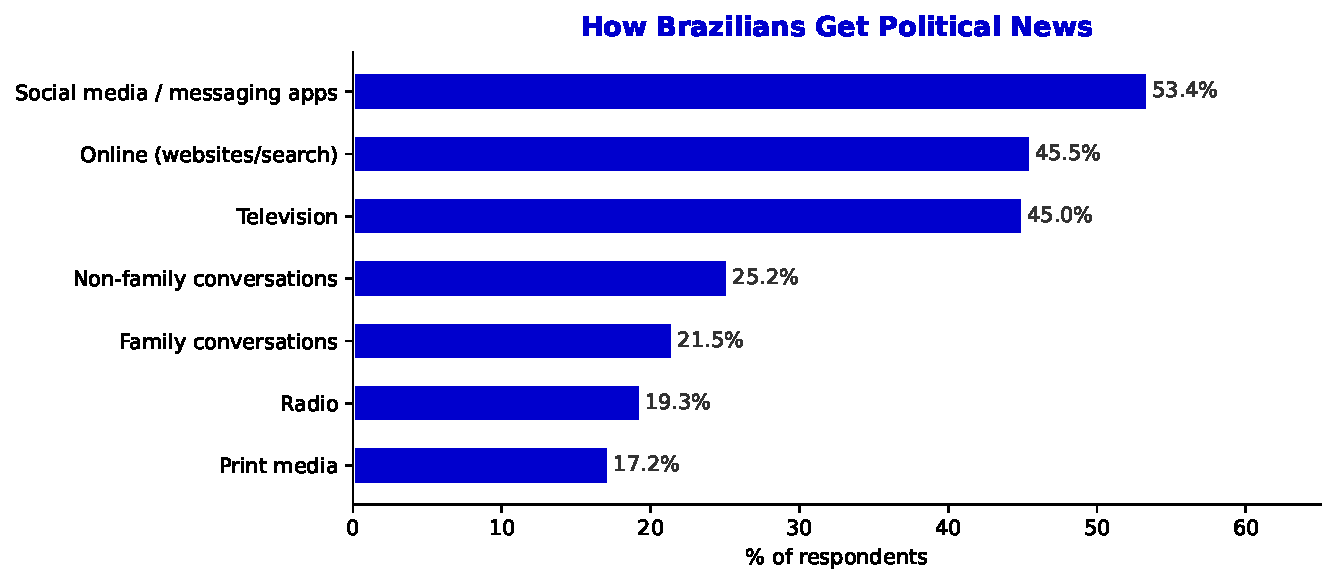
\includegraphics[width=\textwidth]{fig_news_habits.pdf}
    \column{0.38\textwidth}
      \vspace{0.8em}
      \begin{block}{Key finding}
        \textbf{Social media and messaging apps} are the dominant source of political news (53\%), surpassing television and online search.
      \end{block}
      \vspace{0.4em}
      \begin{exampleblock}{Implication}
        WhatsApp groups are the primary arena for political conflict — making them the right target for citizen-level interventions.
      \end{exampleblock}
  \end{columns}
\end{frame}

\begin{frame}{Platforms for Political Content}
  \begin{columns}[T]
    \column{0.58\textwidth}
      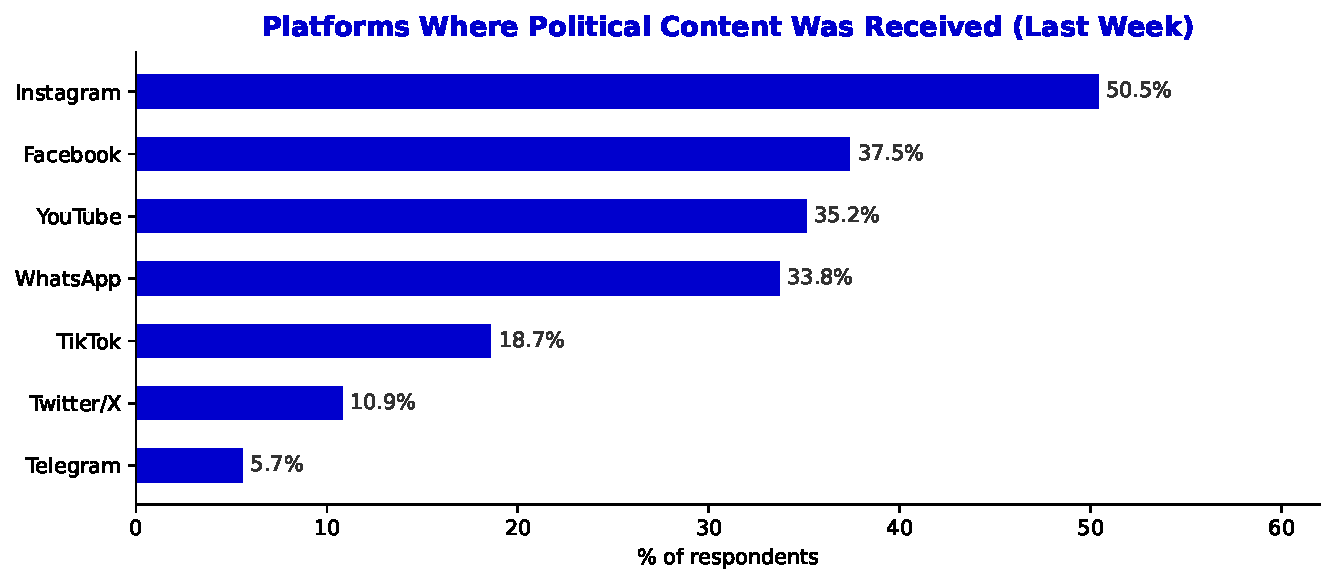
\includegraphics[width=\textwidth]{fig_platforms.pdf}
    \column{0.38\textwidth}
      \vspace{0.8em}
      \textbf{Instagram leads} (50.5\%), followed by Facebook (37.5\%) and WhatsApp (33.8\%).\\[8pt]
      Twitter/X (10.9\%) and Telegram (5.7\%) remain niche.\\[8pt]
      \begin{block}{Design relevance}
        Instagram + Facebook coverage justifies Meta ad targeting for the \textbf{elite experiment}.
      \end{block}
  \end{columns}
\end{frame}

\begin{frame}{Frequency of Active Political Content Seeking}
  \begin{center}
    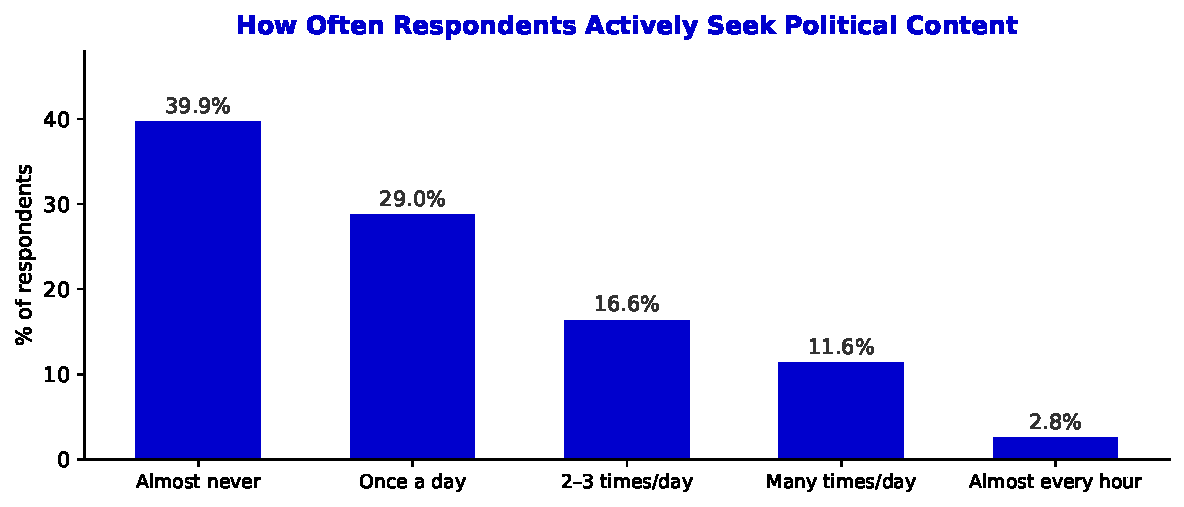
\includegraphics[width=0.78\textwidth]{fig_freq_content.pdf}
  \end{center}
  \vspace{-0.3em}
  {\footnotesize Nearly 70\% actively seek political content at least once a day. High political engagement → high treatment reachability.}
\end{frame}

\begin{frame}{Exposure to Online Political Conflict}
  \begin{columns}[T]
    \column{0.58\textwidth}
      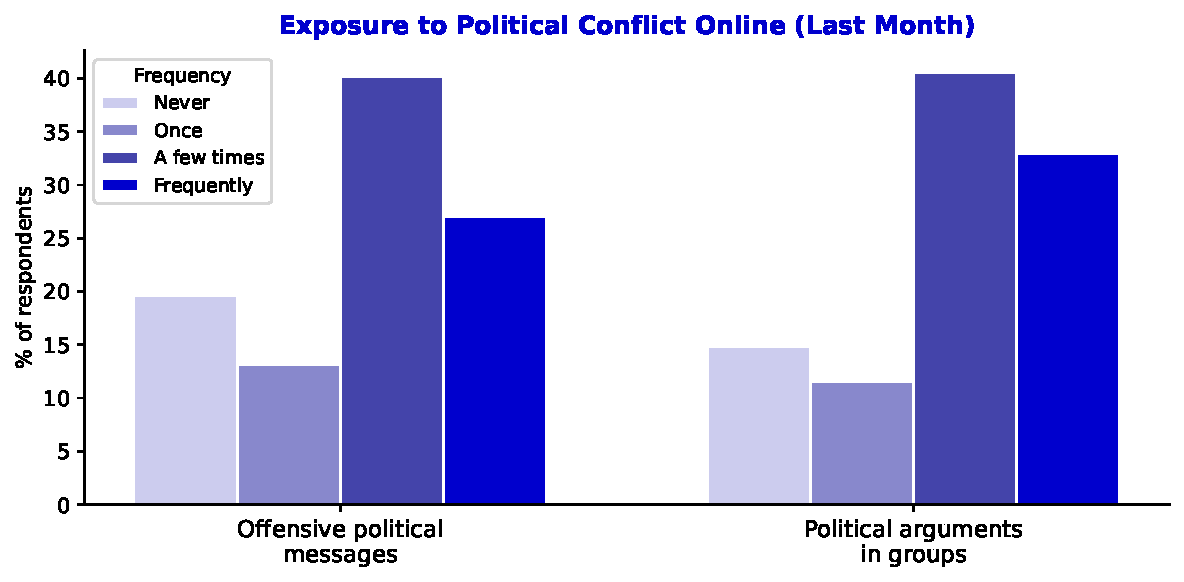
\includegraphics[width=\textwidth]{fig_exposure.pdf}
    \column{0.38\textwidth}
      \vspace{1em}
      \textbf{Conflict is frequent:}
      \begin{itemize}
        \item 67\% saw offensive political messages \emph{a few times or frequently}
        \item 74\% witnessed political arguments in groups at that level
      \end{itemize}
      \vspace{0.4em}
      \begin{alertblock}{Motivation}
        The problem is not latent — it is actively experienced. Concern about polarization is grounded in everyday reality.
      \end{alertblock}
  \end{columns}
\end{frame}

\begin{frame}{Avoidance Behaviors Due to Political Conflict}
  \begin{center}
    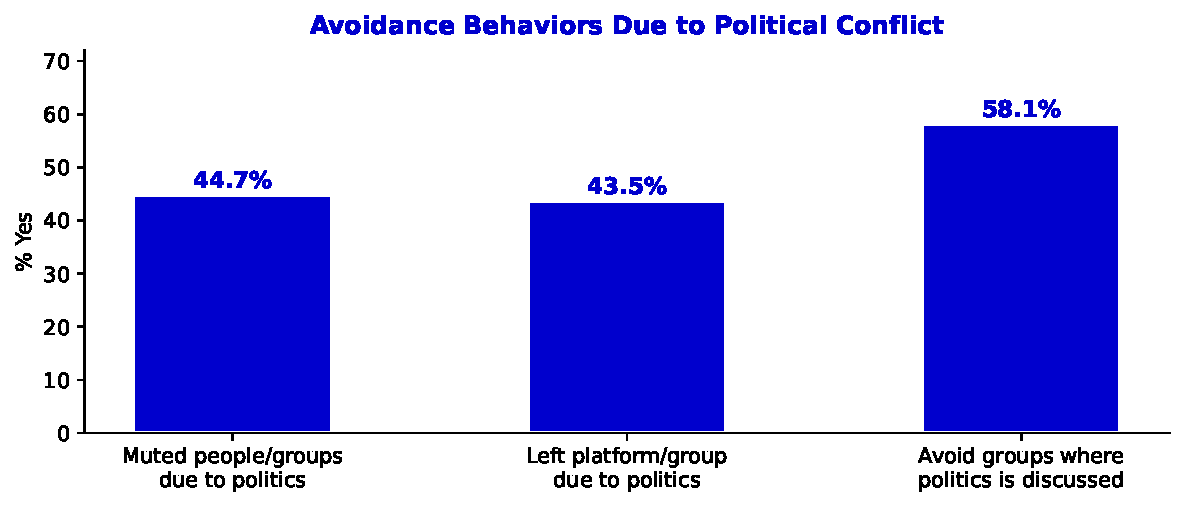
\includegraphics[width=0.78\textwidth]{fig_avoidance.pdf}
  \end{center}
  \vspace{-0.3em}
  {\footnotesize Majorities have taken active steps to disengage from political conflict online. This avoidance — rather than engagement — is the default response our intervention aims to change.}
\end{frame}

\begin{frame}{Affective Polarization: In-group vs.\ Out-group Thermometers}
% x: 1 pt = 0.093 cm (100 pts = 9.3 cm)
% y rows (cm): Antipetistas=3.6, Petistas=1.8, Non-partisans=0.0  (gap=1.8 cm each)
\begin{center}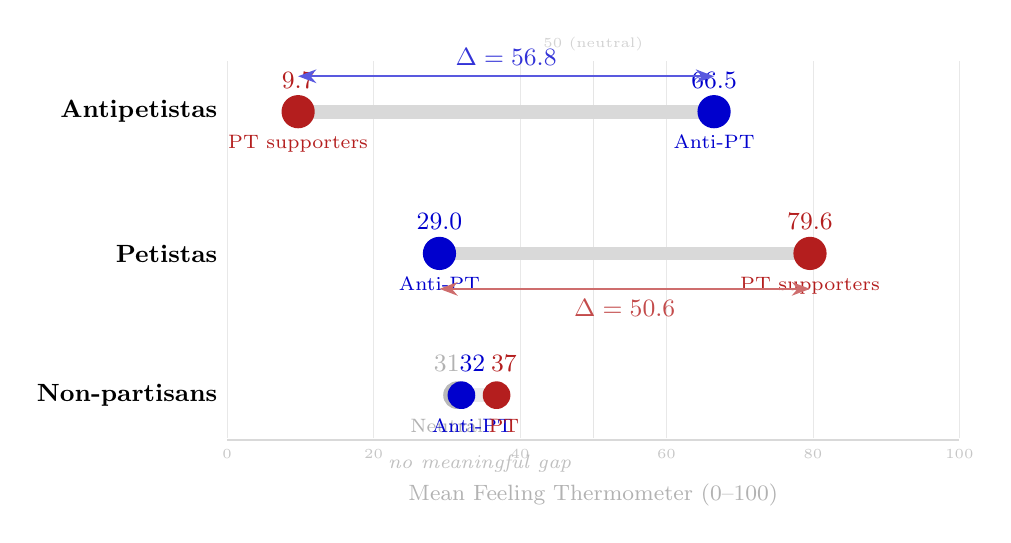
\begin{tikzpicture}[x=0.093cm, y=1.0cm]
  % ── grid ──────────────────────────────────────────────────
  \foreach \xv in {0,20,40,60,80,100}{
    \draw[gray!18, very thin] (\xv,-0.55) -- (\xv,4.25);
    \node[gray!45, font=\tiny, below] at (\xv,-0.57) {\xv};
  }
  \draw[gray!30, thin] (0,-0.57) -- (100,-0.57);
  \draw[gray!20, thin] (50,-0.55) -- (50,4.25);
  \node[gray!35, font=\tiny, above] at (50,4.25) {50 (neutral)};
  \node[font=\footnotesize, gray!60, below] at (50,-1.0)
    {Mean Feeling Thermometer (0--100)};

  % Colors: Petistas/PT = red (IJLred), Antipetistas/Anti-PT = blue (IJLblue)

  % ── Antipetistas  (y = 3.6)  overlay 1 ───────────────────
  \onslide<1->{
    \node[font=\small\bfseries, left] at (0,3.6) {Antipetistas};
    \draw[gray!30, line width=5pt, line cap=round] (9.7,3.6) -- (66.5,3.6);
    \fill[IJLred]  (9.7,3.6)  circle (6pt);   % out-group: PT = red
    \fill[IJLblue] (66.5,3.6) circle (6pt);   % in-group: Anti-PT = blue
    \node[IJLred,  font=\small, above=5pt] at (9.7,3.6)  {9.7};
    \node[IJLblue, font=\small, above=5pt] at (66.5,3.6) {66.5};
    \node[IJLred,  font=\scriptsize, below=5pt] at (9.7,3.6)  {PT supporters};
    \node[IJLblue, font=\scriptsize, below=5pt] at (66.5,3.6) {Anti-PT};
  }

  % ── Petistas  (y = 1.8)  overlay 2 ───────────────────────
  \onslide<2->{
    \node[font=\small\bfseries, left] at (0,1.8) {Petistas};
    \draw[gray!30, line width=5pt, line cap=round] (29.0,1.8) -- (79.6,1.8);
    \fill[IJLblue] (29.0,1.8) circle (6pt);   % out-group: Anti-PT = blue
    \fill[IJLred]  (79.6,1.8) circle (6pt);   % in-group: PT = red
    \node[IJLblue, font=\small, above=5pt] at (29.0,1.8) {29.0};
    \node[IJLred,  font=\small, above=5pt] at (79.6,1.8) {79.6};
    \node[IJLblue, font=\scriptsize, below=5pt] at (29.0,1.8) {Anti-PT};
    \node[IJLred,  font=\scriptsize, below=5pt] at (79.6,1.8) {PT supporters};
  }

  % ── Non-partisans  (y = 0.0)  overlay 3 ──────────────────
  \onslide<3->{
    \node[font=\small\bfseries, left] at (0,0.0) {Non-partisans};
    \draw[gray!15, line width=5pt, line cap=round] (31.4,0.0) -- (36.8,0.0);
    \fill[gray!55]  (31.4,0.0) circle (5pt);
    \fill[IJLblue]  (32.0,0.0) circle (5pt);  % Anti-PT = blue
    \fill[IJLred]   (36.8,0.0) circle (5pt);  % PT = red
    \node[gray!60,  font=\small, above=5pt] at (30.0,0.0)  {31};
    \node[IJLblue,  font=\small, above=5pt] at (33.5,0.0)  {32};
    \node[IJLred,   font=\small, above=5pt] at (37.8,0.0)  {37};
    \node[gray!60,  font=\scriptsize, below=5pt] at (30.0,0.0)  {Neutral};
    \node[IJLblue,  font=\scriptsize, below=5pt] at (33.5,0.0)  {Anti-PT};
    \node[IJLred,   font=\scriptsize, below=5pt] at (37.8,0.0)  {PT};
    \node[gray!50,  font=\scriptsize, below=18pt] at (34.5,0.0)
      {\itshape no meaningful gap};
  }

  % ── Gap arrows  (overlay 4) ───────────────────────────────
  \onslide<4->{
    \draw[IJLblue!65, <->, >=Stealth, thick]
      (9.7,4.05) -- node[above, font=\small\bfseries, IJLblue!80]{$\Delta=56.8$}
      (66.5,4.05);
    \draw[IJLred!65, <->, >=Stealth, thick]
      (29.0,1.35) -- node[below, font=\small\bfseries, IJLred!80]{$\Delta=50.6$}
      (79.6,1.35);
  }
\end{tikzpicture}\end{center}
{\footnotesize \textit{Note:} Petistas = PT as favourite party ($n\approx1{,}374$); Antipetistas = PT as least favourite ($n\approx2{,}122$); Non-partisans = all others.}
\end{frame}

% ============================================================
\section{Survey Experiment Design}
% ============================================================

\begin{frame}{Survey Experiment: Five-Wave Panel}
  \begin{center}
  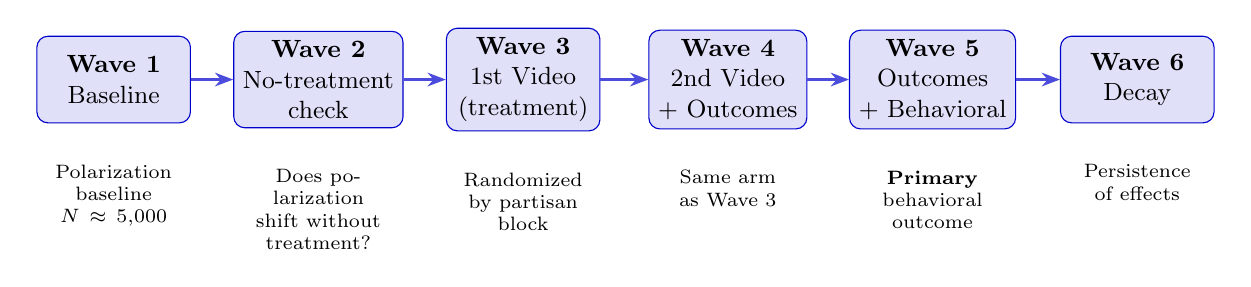
\begin{tikzpicture}[
    wave/.style={rectangle, rounded corners=4pt, draw=IJLblue, fill=IJLblue!12,
                 minimum width=1.95cm, minimum height=1.1cm, align=center, font=\small},
    arrow/.style={-Stealth, thick, IJLblue!70},
    label/.style={font=\scriptsize, align=center, text width=1.95cm}
  ]
    \node[wave] (w1) at (0*2.6, 0)    {\textbf{Wave 1}\\Baseline};
    \node[wave] (w2) at (1*2.6, 0)    {\textbf{Wave 2}\\No-treatment\\check};
    \node[wave] (w3) at (2*2.6, 0)    {\textbf{Wave 3}\\1st Video\\(treatment)};
    \node[wave] (w4) at (3*2.6, 0)    {\textbf{Wave 4}\\2nd Video\\+ Outcomes};
    \node[wave] (w5) at (4*2.6, 0)    {\textbf{Wave 5}\\Outcomes\\+ Behavioral};
    \node[wave] (w6) at (5*2.6, 0)    {\textbf{Wave 6}\\Decay};
    \foreach \i in {1,...,5}{
      \pgfmathtruncatemacro{\j}{\i+1}
      \draw[arrow] (w\i.east) -- (w\j.west);
    }
    \node[below=0.4cm of w1, label] {Polarization\\baseline\\$N \approx 5{,}000$};
    \node[below=0.4cm of w2, label] {Does polarization\\shift without\\treatment?};
    \node[below=0.4cm of w3, label] {Randomized\\by partisan\\block};
    \node[below=0.4cm of w4, label] {Same arm\\as Wave 3};
    \node[below=0.4cm of w5, label] {\textbf{Primary}\\behavioral\\outcome};
    \node[below=0.4cm of w6, label] {Persistence\\of effects};
  \end{tikzpicture}
  \end{center}
  \vspace{0.5em}
  {\small \textbf{Randomization:} block-randomized by partisan group (PT supporters / Anti-PT / Neutral)\\
  \textbf{Retention incentive:} lottery of 3 prizes of 1,000 Korus for panelists completing all waves\\
  Wave 2 has no treatment — it tests whether polarization or issue priorities shift naturally during the campaign.}
\end{frame}

\begin{frame}{Treatment Arms: Four Informational Frames}
  \begin{columns}[T]
    \column{0.48\textwidth}
      \begin{block}{\textcolor{macroC}{Macro Frames}}
        \vspace{0.3em}
        \textbf{Democratic Deterioration}\\
        Polarization undermines electoral trust, weakens institutions, reduces acceptance of outcomes.\\[8pt]
        \textbf{Economic Deterioration}\\
        Polarization increases uncertainty, discourages investment, generates gridlock, slows growth.
      \end{block}
    \column{0.48\textwidth}
      \begin{block}{\textcolor{microC}{Micro Frames}}
        \vspace{0.3em}
        \textbf{Social Conflict}\\
        Polarization increases everyday hostility, normalizes aggression, reduces social trust.\\[8pt]
        \textbf{Family Conflict}\\
        Polarization damages family relationships, causes estrangement and lasting relational harm.
      \end{block}
  \end{columns}
  \vspace{0.6em}
  \begin{center}
    \begin{tabular}{>{\centering\arraybackslash}p{2cm}>{\centering\arraybackslash}p{8cm}}
      \hline
      \textbf{Control} & No informational frame; outcome measurement only \\
      \hline
    \end{tabular}
  \end{center}
  {\small \textit{Note:} Identical content across survey and field experiments.}
\end{frame}

\begin{frame}{Video Placeholder — Wave 2, Democratic Deterioration}
  \begin{center}
    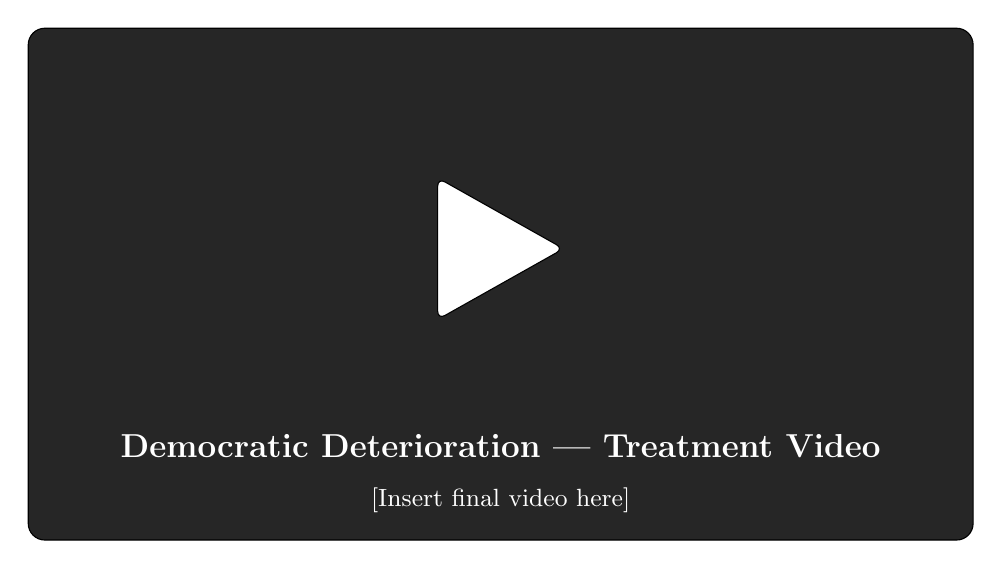
\begin{tikzpicture}
      \draw[fill=black!85, rounded corners=6pt]
        (0,0) rectangle (12,6.5);
      \draw[fill=white!20, rounded corners=3pt]
        (5.2, 2.8) -- (6.8, 3.7) -- (5.2, 4.6) -- cycle;
      \node[white, font=\large\bfseries] at (6, 1.2)
        {Democratic Deterioration — Treatment Video};
      \node[white!70, font=\small] at (6, 0.5)
        {[Insert final video here]};
    \end{tikzpicture}
  \end{center}
\end{frame}

\begin{frame}{Video Placeholder — Wave 2, Economic Deterioration}
  \begin{center}
    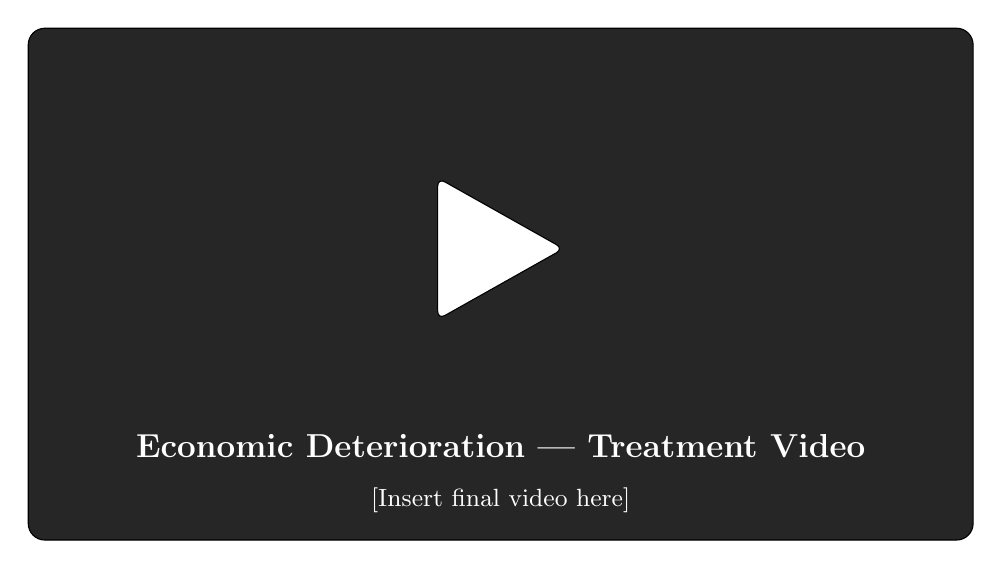
\begin{tikzpicture}
      \draw[fill=black!85, rounded corners=6pt]
        (0,0) rectangle (12,6.5);
      \draw[fill=white!20, rounded corners=3pt]
        (5.2, 2.8) -- (6.8, 3.7) -- (5.2, 4.6) -- cycle;
      \node[white, font=\large\bfseries] at (6, 1.2)
        {Economic Deterioration — Treatment Video};
      \node[white!70, font=\small] at (6, 0.5)
        {[Insert final video here]};
    \end{tikzpicture}
  \end{center}
\end{frame}

\begin{frame}{Video Placeholder — Wave 2, Social Conflict}
  \begin{center}
    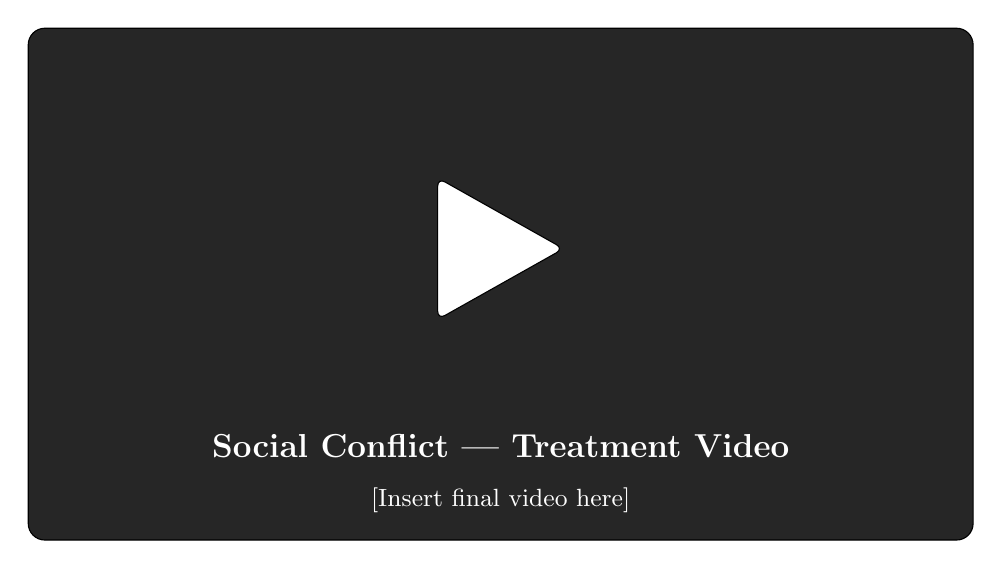
\begin{tikzpicture}
      \draw[fill=black!85, rounded corners=6pt]
        (0,0) rectangle (12,6.5);
      \draw[fill=white!20, rounded corners=3pt]
        (5.2, 2.8) -- (6.8, 3.7) -- (5.2, 4.6) -- cycle;
      \node[white, font=\large\bfseries] at (6, 1.2)
        {Social Conflict — Treatment Video};
      \node[white!70, font=\small] at (6, 0.5)
        {[Insert final video here]};
    \end{tikzpicture}
  \end{center}
\end{frame}

\begin{frame}{Video Placeholder — Wave 2, Family Conflict}
  \begin{center}
    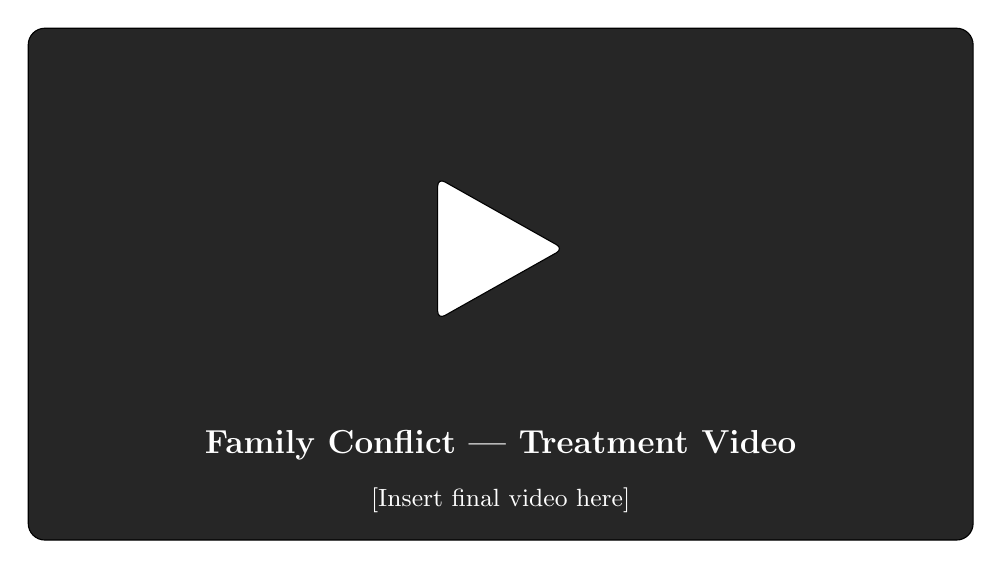
\begin{tikzpicture}
      \draw[fill=black!85, rounded corners=6pt]
        (0,0) rectangle (12,6.5);
      \draw[fill=white!20, rounded corners=3pt]
        (5.2, 2.8) -- (6.8, 3.7) -- (5.2, 4.6) -- cycle;
      \node[white, font=\large\bfseries] at (6, 1.2)
        {Family Conflict — Treatment Video};
      \node[white!70, font=\small] at (6, 0.5)
        {[Insert final video here]};
    \end{tikzpicture}
  \end{center}
\end{frame}

\begin{frame}{Primary Behavioral Outcomes}
  \begin{columns}[T]
    \column{0.48\textwidth}
      \begin{block}{Primary: Seminar Enrollment}
        \vspace{0.3em}
        After treatment, respondents are offered free enrollment in a \textbf{1-hour online seminar} organized by \emph{Redes Cordiais}:
        \begin{itemize}
          \item Practical strategies for polarizing content
          \item Responding to misinformation
        \end{itemize}
        \vspace{0.3em}
        \textbf{Enrollment click = primary outcome}
      \end{block}
    \column{0.48\textwidth}
      \begin{block}{Secondary: Manual Download}
        \vspace{0.3em}
        Respondents are offered a downloadable \textbf{practical manual} with tips for managing political conflict in WhatsApp groups.\\[6pt]
        Download click = secondary behavioral outcome
      \end{block}
      \vspace{0.4em}
      \begin{exampleblock}{Why behavioral?}
        \small Both outcomes require active choice, not just stated willingness. Low cost \& low social desirability bias.
      \end{exampleblock}
  \end{columns}
\end{frame}

\begin{frame}{Secondary Outcomes and Mechanisms}
  \begin{columns}[T]
    \column{0.48\textwidth}
      \textbf{Secondary outcomes (voters)}
      \begin{itemize}
        \item Stated willingness to intervene in WhatsApp conflicts
        \item Self-reported corrective behavior (subsequent waves)
        \item Support for democratic norms / election acceptance
        \item Affective thermometers (H7 ``should not move'')
      \end{itemize}
      \vspace{0.5em}
      \textbf{Mechanisms}
      \begin{itemize}
        \item Perceived costs of polarization (macro index, micro index)
        \item Perceived efficacy of intervention
        \item Perceived social cost of speaking up
      \end{itemize}
    \column{0.48\textwidth}
      \textbf{Placebo / ``Should not move''}
      \begin{itemize}
        \item Partisan compromise attitudes
        \item Anti-democratic norm trade-offs (e.g., bypassing courts)
        \item Affective polarization thermometers
      \end{itemize}
      \vspace{0.4em}
      \begin{alertblock}{H7 test}
        If behavioral outcomes move \emph{without} thermometers moving, we confirm action $\neq$ attitude change.
      \end{alertblock}
  \end{columns}
\end{frame}

% ============================================================
\section{Hypotheses}
% ============================================================

\begin{frame}{Pre-Registered Hypotheses}
  \begin{center}
  \renewcommand{\arraystretch}{1.4}
  \begin{tabular}{>{\bfseries}p{0.8cm} p{10.5cm}}
    \toprule
    H1 & \textbf{Manipulation check:} Each treatment increases perceived costs of polarization in its corresponding domain (macro vs.\ micro). \\
    \midrule
    H2 & Exposure to any treatment \textbf{reduces polarizing rhetoric} among candidates relative to control. \\
    H3 & Exposure to any treatment \textbf{increases behavioral engagement} among voters relative to control. \\
    \midrule
    H4 & \textcolor{macroC}{\textbf{Macro frames}} produce larger effects among \textbf{candidates} than micro frames. \\
    H5 & \textcolor{microC}{\textbf{Micro frames}} produce larger effects among \textbf{voters} than macro frames. \\
    \midrule
    H6 & Treatment effects are \textbf{mediated} by increased perceived costs and perceived efficacy. \\
    H7 & Behavioral effects may occur \textbf{without significant changes} in affective polarization. \\
    \bottomrule
  \end{tabular}
  \end{center}
\end{frame}

% ============================================================
\section{Results: Voter Survey}
% ============================================================

% ============================================================
\section{Field Experiment: Elite Candidates}
% ============================================================

\begin{frame}{Field Experiment: Targeting Political Elites}
  \begin{columns}[T]
    \column{0.52\textwidth}
      \textbf{Population \& Scale}
      \begin{itemize}
        \item $\sim$10,000 candidates for Federal and State Deputy
        \item Identified via official electoral records (TSE)
        \item Verified public Meta accounts (Facebook \& Instagram)
        \item \textbf{Over 25,000 candidate emails extracted} from official records
      \end{itemize}
      \vspace{0.4em}
      \textbf{Delivery}
      \begin{itemize}
        \item Paid Meta advertisements shown in candidates' own social media environments
        \item Direct email campaign with treatment videos
        \item Individual-level randomization (5 arms)
      \end{itemize}
    \column{0.44\textwidth}
      \begin{block}{Outcome Measurement}
        \vspace{0.3em}
        \textbf{Polarizing rhetoric} in public posts during campaign period, measured via \textbf{supervised text classification}:
        \begin{itemize}
          \item Delegitimizing opponents
          \item Framing rivals as threats
          \item Inflammatory language
        \end{itemize}
      \end{block}
      \vspace{0.3em}
      \begin{exampleblock}{Secondary}
        Depolarizing cues (civility, bridge-building) and democratic norm compliance
      \end{exampleblock}
  \end{columns}
\end{frame}

\begin{frame}{Partnership with Redes Cordiais}
  \begin{columns}[T]
    \column{0.52\textwidth}
      \textbf{Who they are}
      \begin{itemize}
        \item Leading Brazilian NGO focused on online conflict de-escalation
        \item Experience training citizens to respond to polarizing content
        \item Recognized credibility across political groups
      \end{itemize}
      \vspace{0.5em}
      \textbf{Role in the study}
      \begin{itemize}
        \item Co-host of the 1-hour intervention seminar (primary behavioral outcome)
        \item Provide the practical manual for WhatsApp conflict
        \item Lend legitimacy to the intervention materials
      \end{itemize}
    \column{0.44\textwidth}
      \begin{block}{Why this partnership matters}
        \vspace{0.3em}
        The behavioral outcome is not hypothetical — enrollment links to a \textbf{real, existing program}. This eliminates demand effects and ensures the intervention has downstream real-world impact beyond the experiment.
      \end{block}
      \vspace{0.4em}
      \begin{alertblock}{Agreement status}
        \vspace{0.2em}
        Formal agreement with Redes Cordiais in place for seminar delivery and content collaboration.
      \end{alertblock}
  \end{columns}
\end{frame}

\begin{frame}{Elite Experiment: Showing Voters Dislike Polarization}
  \begin{columns}[T]
    \column{0.52\textwidth}
      \textbf{The mechanism for elites}
      \begin{itemize}
        \item Candidates face electoral incentives
        \item Treatment reveals a \textbf{credible signal}: voters are concerned about polarization's costs
        \item Provides reputational \& governance rationale to moderate rhetoric
      \end{itemize}
      \vspace{0.5em}
      \textbf{Campaign channels}
      \begin{enumerate}
        \item Instagram \& Facebook paid ads (Meta targeting by candidate account)
        \item Direct email with treatment videos to 25,000+ candidate emails
        \item Content mirrors the four informational frames used in the survey experiment
      \end{enumerate}
    \column{0.44\textwidth}
      \begin{block}{Key message to elites}
        \vspace{0.3em}
        ``Brazilian voters across the spectrum are concerned about how polarization harms [democracy / the economy / families / communities]. Your rhetoric affects these outcomes.''
      \end{block}
      \vspace{0.4em}
      \begin{exampleblock}{Identification advantage}
        Simultaneous elite + citizen intervention allows testing whether \textbf{supply and demand changes reinforce each other}.
      \end{exampleblock}
  \end{columns}
\end{frame}

% ============================================================
\section{Conclusion}
% ============================================================

\begin{frame}{Summary}
  \begin{columns}[T]
    \column{0.48\textwidth}
      \textbf{What we are doing}
      \begin{enumerate}
        \item 5-wave panel survey experiment with $N \approx 5{,}000$ Brazilian voters
        \item Field experiment with $\sim$10,000 candidates for Federal and State Deputy
        \item Four informational frames (macro: democratic, economic; micro: social, family conflict)
        \item Behavioral primary outcomes (seminar enrollment, manual download)
      \end{enumerate}
    \column{0.48\textwidth}
      \textbf{Why it matters}
      \begin{itemize}
        \item Tests whether \emph{framing} polarization costs is enough to trigger action — without requiring attitude change
        \item First study to intervene simultaneously on both elites and citizens using identical frames
        \item Real-world partnership with Redes Cordiais ensures external validity
        \item Results speak to the possibility of \textbf{behavioral depolarization} even in highly divided polities
      \end{itemize}
  \end{columns}
  \vspace{0.8em}
  \begin{center}
    \begin{exampleblock}{\centering Core contribution}
      \centering
      Concern about polarization is widespread. AWARE tests whether it can be converted into action.
    \end{exampleblock}
  \end{center}
\end{frame}

\end{document}
